
\chapter{Experimental Setup}
\label{sec:ExpSetup}
\chaptermark{Experimental Setup}
To look for BSM physics, we want to create new massive particles.  
For this, we collide lighter particles at a high energy.  
The energy released in the collision can manifest in more massive particles due to the concept of mass-energy equivalence (E=m$\mathrm{c^2}$).
The collision may create one of these new particles, and from it's decay products an experimenter can reconstruct the properties of BSM physics that created the massive state.  

For the measurements presented in this thesis, we collide high energy proton beams,  
which are designed to produce a high collision energy in comparison to fixed-target or electron-positron collisions.    
   
\section{Luminosity and Cross Section}
\label{sec:LumiXsec}
To understand how many occurrences of any physical process to expect in a set of collisions, we need to define at a minimum the concepts of luminosity, L, and cross section, $\sigma$.

The cross section of a process is a measurement of how likely a collision will result in the process of interest.  
The phrase cross section refers to the physical cross section of a classical target and is thus measured in units of area.  
In a high energy collision, the cross section no longer refers to the physical dimensions of the target, and can be calculated directly from Feynman diagrams.  
The areas associated with these cross sections is very small and is measured in barns (b), which is $10^{-28} m^2$.  
BSM physics signatures have cross sections that are generally on the order of picobarns (pb) or femptobarns (fb).  
The process cross section is highly dependent of the energy of the collision and is why it is very important to have large, high energy accelerators for the discovery of new physics.  
The cross section of some SM processes are shown in Figure \ref{figs:SMxsecs}.


\begin{figure}
\begin{center}
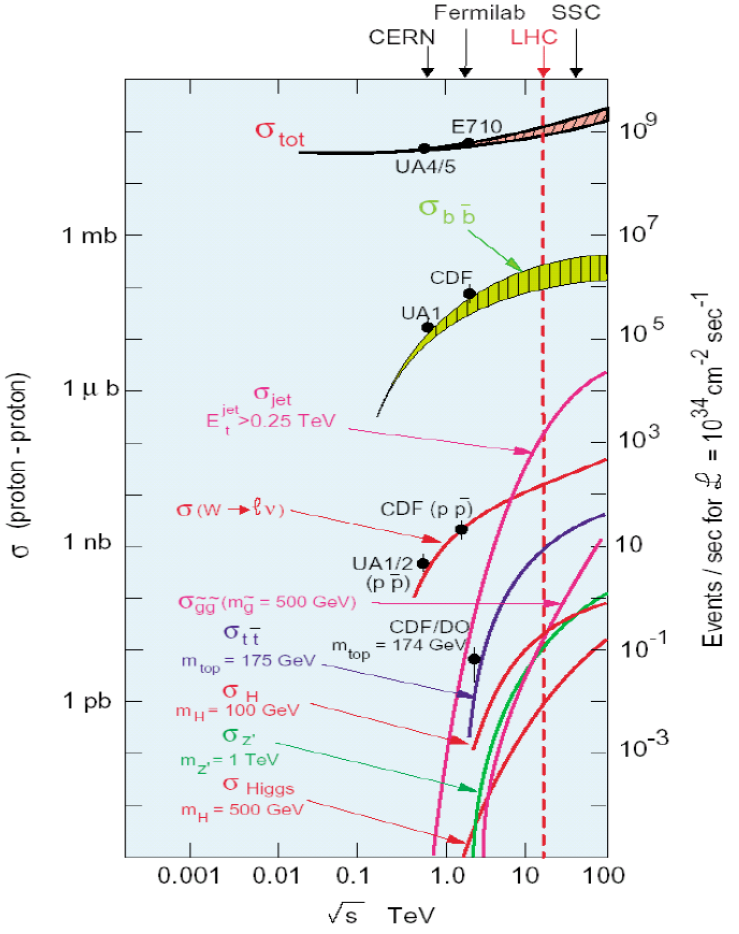
\includegraphics[width=1.0\linewidth]{figs/SMxsecs.png}
\caption{Standard model cross sections as a function of collision energy.}
\label{figs:SMxsecs}
\end{center}
\end{figure}


  
Luminosity is a measure of the intensity of the colliding beams and is the number of collisions expected per unit time per unit area.  
To look for BSM physics, we need to collect an ensemble of useful collisions (events), and thus higher luminosity leads to a larger ensemble and higher statistical precision.  
Additionally, collecting data over time leads to a larger ensemble, so the time-integrated luminosity is a more useful variable to describe the total amount of data collected, 
which is reported in $\fbinv$.  Given in relevant collider properties, the luminosity can be defined as: 
\begin{eqnarray}
\mathrm{L = \frac{\gamma f k_{B} N_{p}^{2}}{4 \pi \epsilon \beta^{*}} F}
\end{eqnarray}  

where $\gamma$ is the Lorentz factor,  f is the frequency of revolution, $k_{B}$ is the number of bunches in the beam, $N_{p}$ is the number of protons per bunch, 
$\epsilon$ is the transverse emittance, $\beta^{*}$ is the betatron function, and F is a reduction factor based on the crossing angle.  

With these two concepts we can extract the predicted number of events for a given process, $N_{\mathrm{i}}$: 
\begin{eqnarray}
N_{\mathrm{i}} = \int L \mathrm{d}t \times \sigma_{\mathrm{i}} 
\label{eqn:Nevents}
\end{eqnarray}  

\section{The LHC}
The Large Hadron Collider (LHC) is a particle accelerator designed to reach collisions energies far surpassing any previous design.  
The LHC is a synchrotron that accelerates protons to 99.999997\% the speed of light.  
These protons beams are then collided at a center-of-mass energy ($\sqrt{s}$) of 8 $\TeV$.  

% http://home.web.cern.ch/about/accelerators
% http://cds.cern.ch/record/1165534/files/CERN-Brochure-2009-003-Eng.pdf

The life of a proton at the LHC starts out as hydrogen gas within the injector of LINAC 2 linear accelerator.  
The atoms are ionized using an electric field, stripping the electron.  
The resulting proton is accelerated using an oscillating electric field.  
The protons are accelerated in a straight line to an energy of 50$\MeV$, or 31\%the speed of light.  

At this energy, linear acceleration is not practical, and the protons enter the Proton Synchrotron Booster (PSB).  
The PSB is composed of four 157 m circumference superimposed synchrotrons that accelerate the protons using electric fields that are synchronized to the revolution frequency of the beams.  
The protons are kept on the circular accelerator with a magnetic field directed into the plane formed by the accelerator ring, which increases in strength as the protons gain energy.  
After the acceleration from the booster, the protons are at en energy of 1.4$\GeV$, or 92\%the speed of light.

After the PSB, the protons enter the Proton Synchrotron (PS), a 628 m circumference synchrotron, which accelerates the protons to 25$\GeV$, or 99.93\%the speed of light.  
After the PS, the protons enter the Super Proton Synchrotron (SPS), a 7 km circumference synchrotron, which accelerates the protons to 450$\GeV$, or 99.9998\%the speed of light.

Finally, the beams enter the LHC.  This is the final synchrotron ring, with a circumference of 27 km.  
After the SPS, the protons are inserted into the LHC in one of two evacuated tunnels depending on which direction around the ring the beam is to travel.  

The LHC uses 1232 dipole magnets to keep the protons in the ring as they accelerate. which provide an 8.3 T field over their length.  
In order to deliver such a field, the magnets use superconducting niobium-titanium cables.  
These cables are cooled by superfluid helium to -271.3 C in order to achieve this superconductivity.  
During each revolution the energy of each proton in the LHC ring increases by 5 MeV.  
After being fully accelerated in the LHC, the protons are at an energy of 4$\TeV$, or 99.999997\%the speed of light.

The proton beams are then directed together for collisions in four positions around the ring.  
Each beam in the LHC ring contains 2808 bunches of protons, and each bunch contains 110 billion protons. 
These bunches need to be collimated in order to maximize collision frequency, which is accomplished by the use of 392 focusing quadrupole magnets.   
Each of these collision points houses its own detector, ALICE (A Large Ion Collider Experiment), ATLAS (A Toroidal LHC Apparatus), 
CMS (Compact Muon Solenoid), and LHCb (Large Hadron Collider beauty).  
The ALICE detector is primarily used for experiments involving heavy ion collisions that expand the current 
understanding of concepts such as the quark-gluon plasma and quark confinement   
LHCb is specialized for physics involving b quarks, such as measuring CP violation parameters from b-hadron interactions.  

CMS and ATLAS are large general purpose detectors.  
These detectors are used for many different types of physics searches, and are the two detectors responsible for the Higgs boson discovery.  
For the purposes of this thesis we will be concentrating on the CMS detector
  
These accelerator segments and detectors can be shown in Figure~\ref{figs:lhc}.

\begin{figure}
\begin{center}
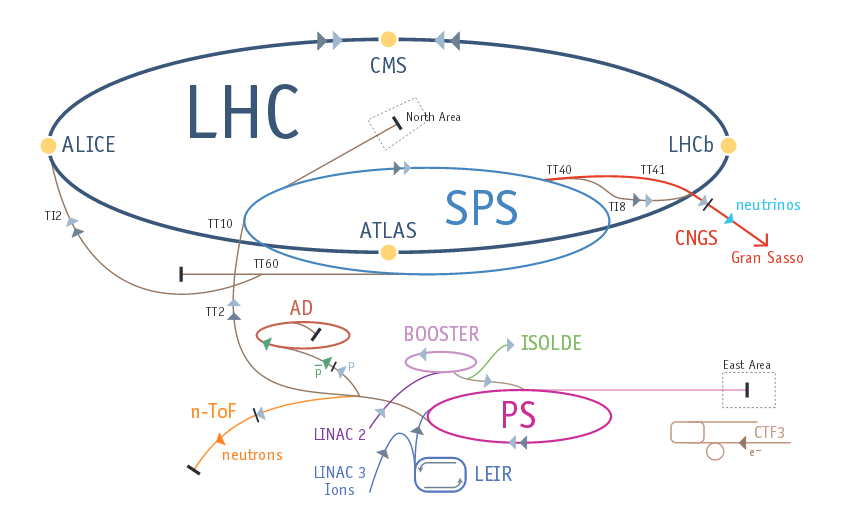
\includegraphics[width=1.0\linewidth]{figs/lhc.png}
\caption{A diagram of the LHC.}
\label{figs:lhc}
\end{center}
\end{figure}
%http://cds.cern.ch/record/1092437/files/CERN-Brochure-2008-001-Eng.pdf

\section{CMS detector}
Here we will detail the basics of the CMS detector subsystems, for a more complete description, see Reference \cite{Bayatian:922757}.
The purpose of the CMS detector is to measure properties of particles that are created in a collision such as the energy and trajectory. 
The detector needs to supply enough information so that particles can be reconstructed and classified.  
Generally, we can reconstruct most physics signatures by analyzing electrons, muons, photon, charged hadrons, and neutral hadrons. 
The CMS detector has dedicated algorithms and systems that are specifically designed to identify each of these categories.  

In order to reconstruct these particles, we impose a uniform axial magnetic field throughout the inner detector with the use of a superconducting magnet. 

The trajectory of charged particles is important to extract information such as charge and momentum.  
The process of reconstructing the trajectory of these  particles is called tracking.  
Near the interaction point tracks are very dense, and tracking becomes very difficult.  
In this region we use a fine array of silicon pixels that register a charge particles position based on charge deposited in the device.  
Additional measurements are made by a second series of silicon detectors called the Silicon Strip Tracker. 
Using a series of these position measurements, we can fit a charged particle track.  

Energy can be measured by the use of calorimeter systems.  
A calorimeter is a detector designed such that a particle will deposit all of its energy within the detector in the form of photons, 
which can be detected to extract a measure of the total energy. 
These systems are subdivided into the Electromagnetic Calorimeter (ECAL) and Hadronic Calorimeter (HCAL).  
The ECAL uses scintillation crystals to detect particles that interact primarily with the electromagnetic force such as electrons and photons.  
Hadrons pass through the ECAL with minimal loss and deposit energy in the HCAL, which uses layers of absorber and scintillator to first 
create a shower of secondary particles, and then measure the total energy of these secondary particles.  

The detection of muons requires a specially designed system that lies outside of the ECAL, HCAL, and magnet.  
Muons pass through the ECAL and HCAL without losing a substantial fraction of their energy.  
To reconstruct the trajectory of muons, we use several different tracking systems both inside and outside the magnet.

See Figure~\ref{figs:CMSdiagram1} for a diagram of the full detector, and Figure~\ref{figs:CMSdiagram} for a cross-sectional view of the detector subsystems.

\begin{figure}
\begin{center}
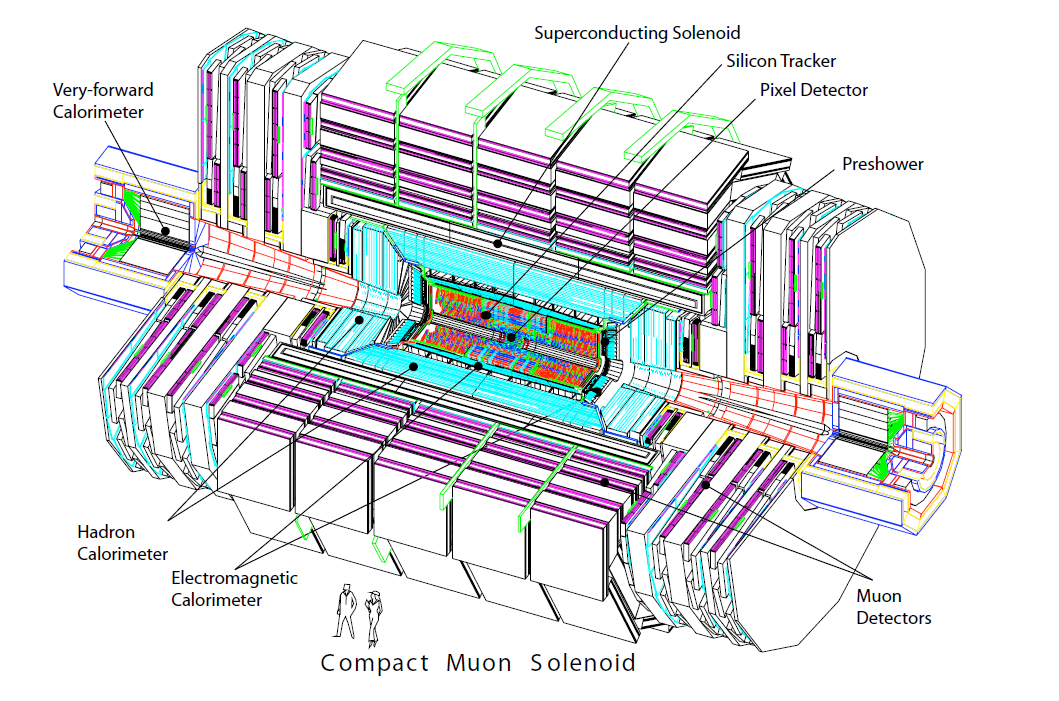
\includegraphics[width=1.0\linewidth]{figs/CMSdiagram1.png}
\caption{A diagram of the full CMS detector.}
\label{figs:CMSdiagram1}
\end{center}
\end{figure}

\begin{figure}
\begin{center}
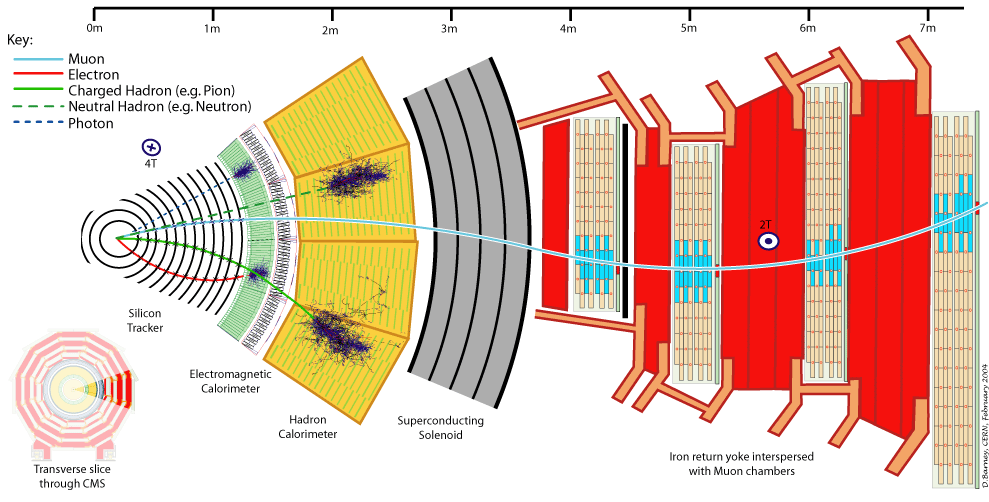
\includegraphics[width=1.0\linewidth]{figs/CMSdiagram.png}
\caption{A cross-sectional view of the CMS detector.}
\label{figs:CMSdiagram}
\end{center}
\end{figure}



\subsection{Pixel Tracker}
The closest detector system to the interaction point is the silicon pixel tracking system.  
This system extends from a radius of 4 cm to 11 cm in the barrel, and is designed to track charged particles in a very dense environment.  
This is achieved with three arrays of two dimensional silicon pixels placed at a radii of 4.4 cm, 7.3 cm, and 10.2 cm, as well as two endcap disks for a total of 65 million pixels.  
When a charged particle traverses one of the 100 $\mum$ $\times$ 150 $\mum$ pixels, it imparts enough energy to the silicon to eject an electron.  
The electrons and their corresponding hole are detected on the pixel surface as a signal.  
This signal allows us to extract a position measurement for the charged particle.  

The entire system exists in a magnetic field, so the trajectory of the electrons and holes are deflected in the r,$\phi$ plane before detection.  
The angle of this Lorentz drift is 23$\textdegree$, which causes the electron-hole pairs to be detected over a wide region covering multiple pixels.  
This effect improves the spacial resolution to 10 $\mum$ in r-$\phi$ space due to the fact that the charge center can be reconstructed by more measurements, 
whereas the z resolution is 20 $\mum$ due to the fact that there is no magnetic deflection in this direction. 
The pixel detectors in the endcap disks are angled at 20$\textdegree$ in a turbine-like design to take advantage of this effect.  

Figure \ref{figs:CMSpixel} shows a diagram of the full pixel detector.    

\begin{figure}
\begin{center}
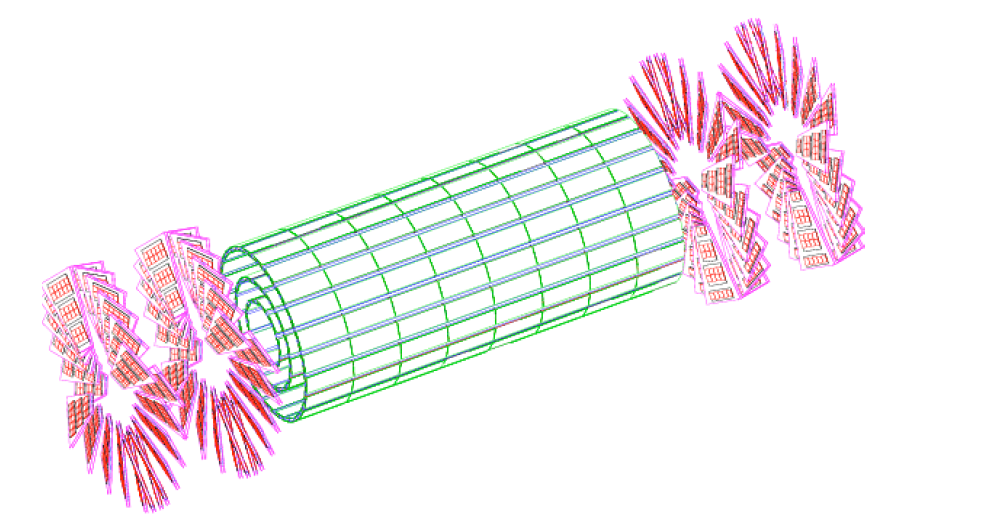
\includegraphics[width=1.0\linewidth]{figs/CMSpixel.png}
\caption{A diagram of the pixel detector.}
\label{figs:CMSpixel}
\end{center}
\end{figure}
  
\subsection{Silicon Strip Tracker}
Outside of the silicon pixel tracker out to a radius of 130 cm in the barrel lies the silicon strip tracking system.  
This system consists ten arrays of silicon strips that work in much the same way as the pixel detectors.  

The system in segmented into the inner barrel, outer barrel, inner disk, and endcap segments.  
The inner barrel segment (20 cm $<$ r $<$ 55 cm) uses four arrays of 10 cm $\times$ 80 $\mum$ silicon microstrips .  
The outer barrel (55 cm  $<$ r $<$ 130 cm) uses six arrays of large pitch 25 cm $\times$ 180 $\mum$ silicon microstrips.  

The endcap silicon strip detector consists of nine disks from 120 cm  $<$ z $<$ 280 cm.  
The inner disk segement contains three smaller disks that connect the inner barrel and endcap segments.  

Figure \ref{figs:CMStracker} shows a diagram of the silicon tracker.    

\begin{figure}
\begin{center}
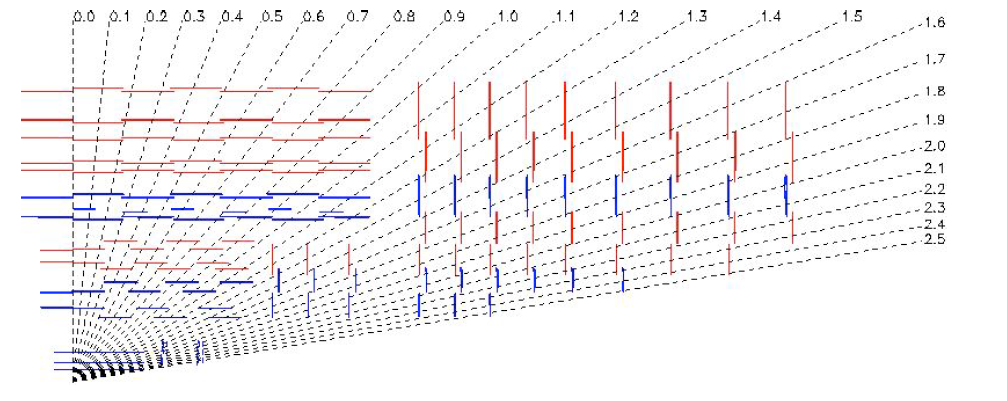
\includegraphics[width=1.0\linewidth]{figs/CMStracker.png}
\caption{A diagram of the silicon tracking system.}
\label{figs:CMStracker}
\end{center}
\end{figure}
  


%\subsection{Preshower Calorimeter}
\subsection{Electromagnetic Calorimeter}
The ECAL is designed to provide energy information for electrons and photons.  
These particles will typically deposit all of their energy within the detector, which is detectable as photons. 

To do this, the ECAL uses 61200 lead tungstate ($\mathrm{PbWO_4}$) scintillation crystals in the barrel and 7324 in each endcap.  
Lead tungstate is chosen as a scintillation material because it has a short radiation length (0.89 cm), fast response (25 ns for 80\% of light), and can 
withstand harsh radiation environments (10 Mrad).
The light emitted is around 30 photons per $\MeV$ for the energy of the particle of interest, which is somewhat low.  
Therefore, the ECAL uses avalanche photodiodes in the barrel and voltage phototriodes in the endcap segments to amplify the signal upon readout.  

The endcap regions of the ECAL include a preshower detector that is used to distinguish high energy photons from decaying pions.  
A pion decaying to two closely spaced photons can mimic one high energy photon to the 2.2 cm wide ECAL crystals.  
The preshower is able to distinguish these events with a finer granularity (2 mm) silicon strip detector.   
 
Figure \ref{figs:CMSecal} shows a diagram of the ECAL.    
\begin{figure}
\begin{center}
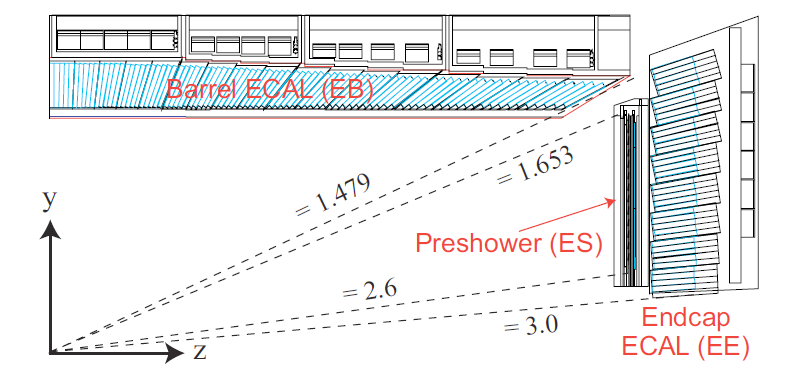
\includegraphics[width=1.0\linewidth]{figs/CMSecal.png}
\caption{A diagram of the ECAL system.}
\label{figs:CMSecal}
\end{center}
\end{figure}
  





\subsection{Hadronic Calorimeter}
The HCAL is designed to give the energy of charged and neutral hadrons, which generally lose very little energy in the ECAL.  
The HCAL is segmented into the inner barrel (inside the magnet), outer barrel (outside the magnet), endcap, and forward (close to the beamline).  

The HCAL uses alternating layers of absorber and scintillator to calculate the energy of these hadrons.  
The absorber creates a cascade of secondary particles that emit photons in the scintillator which can then be detected and summed to reconstruct the energy of the initial hadron.  
The photons emitted in the scintillator are carried to the photodetectors by optical waveguides.  
The HCAL uses hybrid photodiodes to detect the scintillation light and provide a signal that can be used to extract the total energy of the hadron.  

Figure \ref{figs:CMShcal} shows a diagram of the HCAL.   
\begin{figure}
\begin{center}
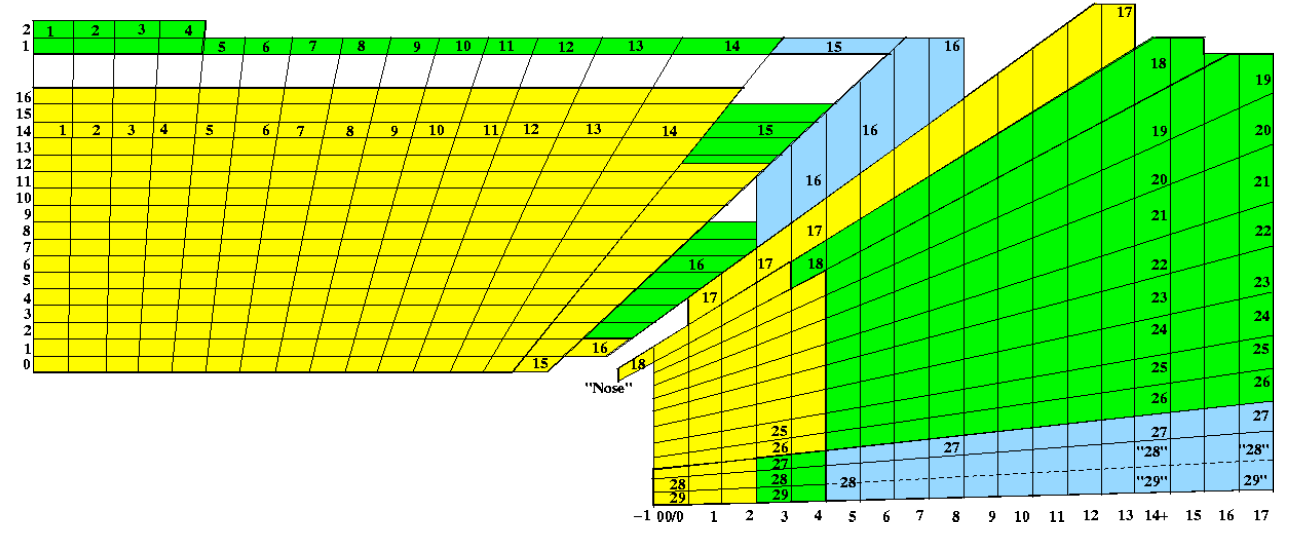
\includegraphics[width=1.0\linewidth]{figs/CMShcal.png}
\caption{A diagram of the HCAL system.}
\label{figs:CMShcal}
\end{center}
\end{figure}
  
\subsection{Magnet}
A charged particle moving perpendicular to a magnetic field follows a helical trajectory.  
The curvature of this helix is dependent on the momentum of the particle, and the handedness is dependent on the charge.  
Therefore, by immersing the tracking volume in an axial magnetic field we can get an accurate measurement of these properties.  
The stronger the magnetic field, the more precise these measurements can be for a high energy particle due to the more distinct curvature.  
To produce this field, CMS employs the largest superconducting magnet ever built.  

The design goal for the magnet is to be able to reproduce high momentum muons.  
The benchmark used for this is to have a momentum resolution of $\Delta$p/p $\leq$ 10\% at a muon momentum of 1 $\TeV$.  
To achieve this, we employ a solenoid with a length of 12.9 m and bore of 5.9 m.  
The coils of this solenoid are superconducting niobium-titanium, which produce a uniform 3.8 T magnetic field in the interior. 
The coils are wound in four layers, for a total of 2168 turns that carry 19.5 kA of current.    

The magnet additionally provides structural support to withstand the weight of the CMS detector as well as the magnetic force exerted from it's own magnetic field.  

\subsection{Muon System}
The reconstruction of muons and electrons starts at the inner silicon tracking system.  
Whereas electrons deposit their energy in the ECAL, a muon will traverse the ECAL and HCAL without significant interaction because a muon is around 200 times as massive.  
Muons are of interest to the Higgs discovery as well as BSM physics, 
and an accurate determination of the muon energy is also required for determination of the total event energy and missing energy.  
Therefore, the CMS detector has a large system purely designed to reconstruct muons, which lies outside all other detector systems at CMS.  

The muon system is comprised of a gaseous detectors interleaved with iron.  
The iron is saturated with the return field of the magnet, which creates a magnetic field at one half of the internal field strength and oriented in the opposite direction.  
The three layers of this ``return yoke" system bends muons to get an accurate measure of the momentum outside of the magnet.  

The trajectory of the muons is reconstructed with three types of gaseous detectors.  
The detectors work on the same basic principle, where an incoming muon ionizes the gas creating an electron-hole pair.  
The electron is detected by the anode, and the hole is detected by a cathode.  
A coincidence of these two measurements gives a measure of the position and time that a muon traversed the detector.  
With a series of these measurements, a trajectory can be fit, and physical quantities of interest can be reconstructed.  

In the barrel region ($|\eta|$ $<$ 1.2), drift tubes are used because the neutron flux and magnetic field are low.  
A drift tube is a detector consisting of a gas filled tube with an anode wire.  
The ionized electron from the gas volume travels to the anode wire, and a measurement of position is made.  
The detection of this electron registers the position along the wire (z coordinate).  
The r-$\phi$ coordinate within the drift tube cross sectional can be calculated by using the drift time of the ionized electrons to the anode.  

In the endcap region, where the magnetic field and neutron flux are high, cathode strip chambers are used.  
Cathode strip chambers are trapezoidal in shape with six gas gaps for ionization.  
These gas gaps each have one plane of cathode strips pointing radially outward and one plane of anode wires oriented perpendicular to the cathode.  

In both the barrel and endcap regions, resistive plate chambers are used.  
These detectors are composed of two parallel resistive plates separated by a gas gap.  
The design goal of the resistive plate chambers is to complement the cathode strip chambers and drift tubes to give two independent measurements of position.  
Additionally, resistive plate chambers offer very quick and accurate time resolution.  This offers a 
quick approximation of the muon momentum which is useful for the trigger system and matching a muon track to a bunch crossing.  

The muon system and inner tracker both contribute to the trajectory measurement of a muon.  
In terms of momentum resolution, the inner tracker offers much better sensitivity up to around 200 $\GeV$.  
After 200 $\GeV$, the muon system starts to significantly improve the momentum measurement.

Figure \ref{figs:CMSmuon} shows a diagram of the muon system.  
\begin{figure}
\begin{center}
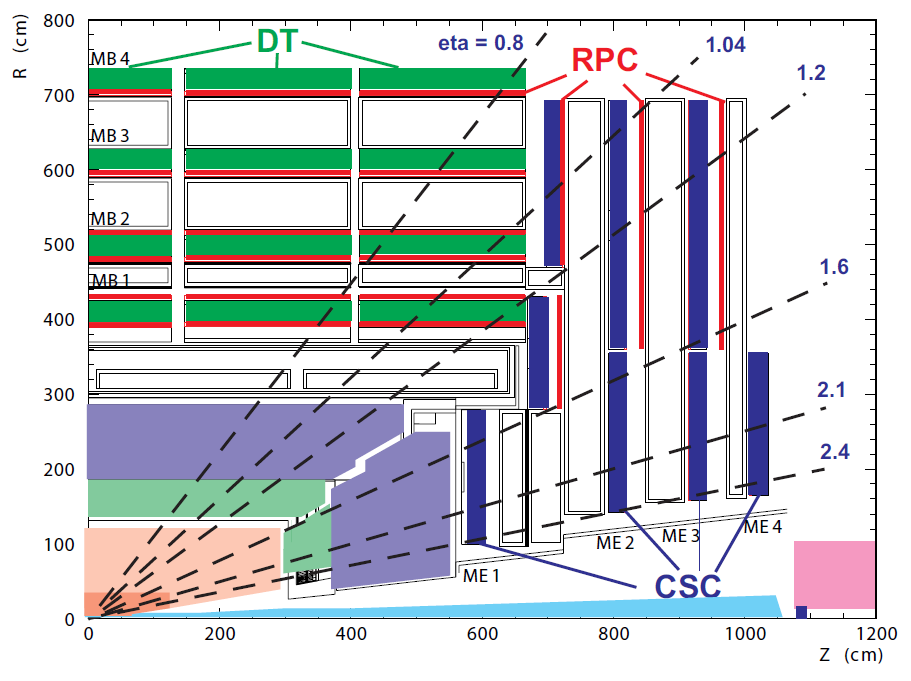
\includegraphics[width=1.0\linewidth]{figs/CMSmuon.png}
\caption{A diagram of the muon system.}
\label{figs:CMSmuon}
\end{center}
\end{figure}

\subsection{Trigger}
The LHC delivers around 1 billion proton-proton collisions per second.  
However, because of the current computing limitations, the CMS detector system can only write around 100 collisions per second as data.  
Therefore, a trigger system is developed to distinguish the most potentially interesting physics signatures.  

The L1 trigger takes information from the calorimeter and muon systems and their correlations.  
When one of these detectors produces a signal, the information takes 3.2 $\mus$ to reach the L1 processing area and return to the detector.  
The L1 processing time for the information for a maximum of 1 $\mus$ where the decision is made to keep the event to search for potential physics signatures.  
The L1 has various algorithms designed to keep ``trigger primitives", which can be objects such as high $\pt$ muons, electrons, jets or full event information like total energy or $\MET$.  
The L1 trigger only saves on average of 1 out of every 1000 events.  

After the L1 trigger, the trigger primitive events are processed by the high level trigger (HLT).  
The HLT again saves only 1 out of 1000 of these events.  
The processing time for the HLT algorithm is longer than the L1 system, and to extract the potentially exciting physics objects the algorithm performs partial event reconstruction.  
An event that enters the HLT algorithm is first analyzed based on the output of the calorimeters and muon system, then pixel tracking is performed, then finally full tracking.  
An event that passes the L1 and HLT is then put into storage for analysis.  

%\subsection{Computing Grid}


